% main.tex, to be used with thesis.tex
% This contains the main work of your thesis.

%\bibliography{thesis}  % uses the references stored in Chapter1Radar.bib

\chapter{Proposal of a Data Persistence in Sensor Networks Taxonomy}
\label{chap:taxonomies}

As revailed in the previous chapter, data persistence for sensor
networks require an understanding of not only the properties of the
infrastructure of a given sensor network, but also of the properties and nature
of the collected data themselves. To put things differently, in order to
identify these concepts more clearly, each section of this chapter proposes an
individual taxonomy based on the aspects described in the literature
review. Then, it briefly discusses the relationships among them.

A taxonomy is defined as the practice and science of classification and uses
the taxonomic units of ``taxa'', the plural form of ``taxon''. Similarly, they
are represented by a hierarchy diagram that relates the main taxonomy to the
different taxa and their own related ones, if any.

\section{Purpose of the Sensor Data Taxonomy}

As delineated in section \ref{sec:sn-data-purpose}, the purpose of the
collected data from sensor devices determines how the collected data is
retrieved and used in the network. In such a fashion, this taxonomy relates to
how the collected data is used, and should be the primary question to be
answered during the analysis of a sensor network. The taxa related to this
taxonomy, depicted in Figure \ref{fig:taxonomy-data-purpose}, is described as
follows:

\begin{figure}[h]
  \centering
  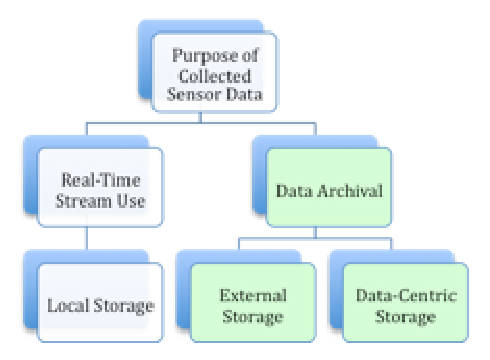
\includegraphics{../diagrams/taxonomy-data-purpose}
  \caption{The Purpose of Sensor Data Taxonomy}
  \label{fig:taxonomy-data-purpose}
\end{figure}

\begin{itemize}
  \item \textbf{Real-time Data Stream}: the collected data is accessed
  on-the-fly from the sensor device as a real-time data stream, and may have a
  short life cycle as it temporarily resides in memory;
  \item \textbf{Data Archival}: the collected data is used for historical
  purposes and is related to the historical data analysis \cite{sn-intro01,
  sn-intro02} or Information Fusion \ref{sn-info-fusion}. 
\end{itemize}

\section{The Location of the Sensor Data Taxonomy}

The location where the collected data is stored plays an important role
in the different aspects of the access to the collected data from sensor
devices, as shown in section \ref{sec:sn-storage-locations}. In this way,
Figure \ref{fig:taxonomy-data-location} depicts this taxonomy, which can be
described as follows:

\begin{figure}[h]
  \centering
  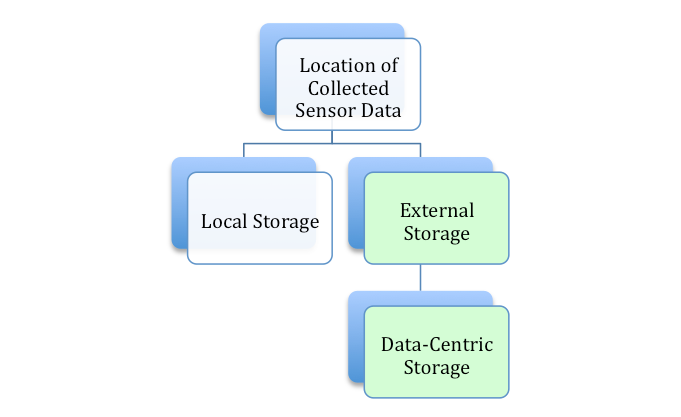
\includegraphics{../diagrams/taxonomy-data-location}
  \caption{The Location of Sensor Data Taxonomy}
  \label{fig:taxonomy-data-location}
\end{figure}

\begin{itemize}
  \item \textbf{Local Storage}: characterizes the placed of the collected data
  temporarily located in-memory, or in a secondary storage device on a node
  located in-network;
  \item \textbf{External Storage}: The collected data is usually located in an
  external storage device with a data management system such as a relational
  database;
  \item \textbf{Data-Centric Storage}: when the collected data occupies
  different external storages, being organized by categories based on the
  collected data keys and values. In other words, what characterizes this taxon
  is the presence of a data partitioning strategy to store the collected data.
\end{itemize}

\section{Data Model Taxonomy}

One of the fundamental challenges in the development of a persistence storage
in sensor networks is related to the data model chosen to represent the
collected data. Different data models were reported in the review of related
literature in section \ref{sec:data-models}. As a consequence, this taxonomy
relates to the data model used to design the collected data, as drawn in Figure
\ref{fig:taxonomy-data-model}, and described as follows.

\begin{figure}[h]
  \centering
  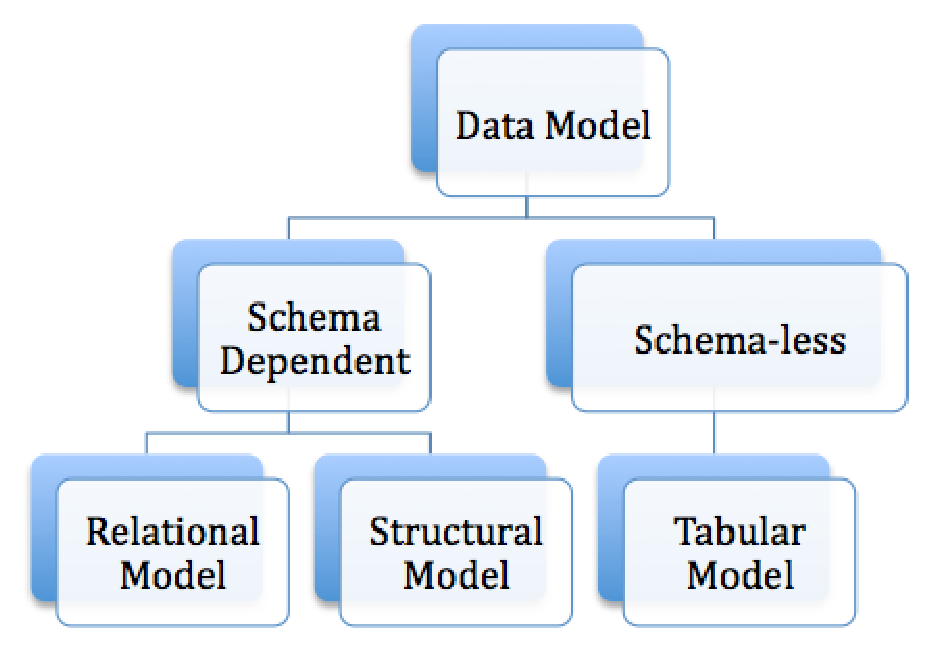
\includegraphics{../diagrams/taxonomy-data-model}
  \caption{Data Model Taxonomy}
  \label{fig:taxonomy-data-model}
\end{figure}

\begin{itemize}
  \item \textbf{Schema-Dependent Models}: this data model requires the
  definition of a master schema that describes the data through a rigorous of 
  data modeling process prior to the insertion of the data. Examples of such
  model is the traditional Relational Data Model\cite{relational-model}, as
 well as the Structured Data Models such as the XML \cite{xml};
  \item \textbf{Schema-less Models}: contrary to the former taxon, schema-less
  data models do not require the definition of a data schema or table
  definition. Instances of such data model reviewed in the literature review
  is the use of the Tabular Data model.
\end{itemize}

\section{Data Provenance Taxonomy}

No matter which data model used to represent the collected data, Data
Provenance provides a valuable guideline on how to describe the collected data
from sensors devices. As reported in section \ref{sec:sn-provenance}, the
description of the properties should take into account different properties of
the nature of the data as shown in Figure \ref{fig:taxonomy-data-provenance}.
Those taxa are summarized as follows:

\begin{figure}[h]
  \centering
  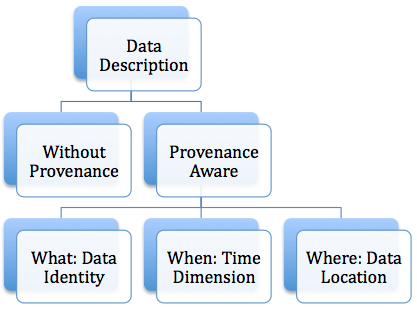
\includegraphics{../diagrams/taxonomy-data-provenance}
  \caption{Data Provenance Taxonomy}
  \label{fig:taxonomy-data-provenance}
\end{figure}

\begin{itemize}
  \item \textbf{What: Data Identity}: the data type that uniquely identifies
  the collected data from sensors. First and foremost, the properties of the
  sensor devices must be described according to the meaningful naming
  convention for the property. For instance, ``Water Temperature'' better
  describes the intent of the property as ``temp''. Second, the identification
  of the collected data related to the sensor type should be given, that is,
  which sensor device created the collected data, in case the data origin is
  relevant;
  \item \textbf{When: Time Dimension}: time is an important attribute of the
  data because it identifies the age of the collected data. Depending on the 
  use of the collected data, this is often taken into account. Two different
  types of time dimensions were described: \textbf{fact} and
  \textbf{transaction} times. The former is used to identify when the data
  was collected, whereas the latter when the data was transmitted to the
  data sink where the query processing acts;
  \item \textbf{Where: Data Location}: the point where the collected data was
  observed by the sensor device. Usually the latitude and longitude as the GPS
  coordinates are provided by devices which are capable of sensing the
  location. A descriptive metadata about the location could also be given such
  as room-name = ``deep see''.
\end{itemize}

\section{Query Processing Mechanism Taxonomy}

The query processing mechanism in sensor networks is directly related to how
and where the collected data is used and stored, as shown in section
\ref{sec:query-process}. As a consequence, the following taxa are related to the
different types of query processing mechanisms and summarized in Figure
\ref{fig:taxonomy-query-mechanism}:

\begin{figure}[h]
  \centering
  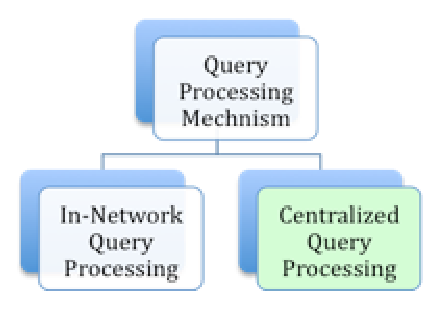
\includegraphics{../diagrams/taxonomy-query-mechanism}
  \caption{Query Processing Mechanism Taxonomy}
  \label{fig:taxonomy-query-mechanism}
\end{figure}

\begin{itemize}
  \item \textbf{In-Network Query Processing}: when the data node is the
  sensor device itself, and it uses the local storage mechanism, then the
  sensor node is able to reply to request related to the observations of the 
  environment defined by the sensor device. In this way, the query takes 
  place in the network itself, and usually returns values related to the current
  state of the environment;
  \item \textbf{Centralized Query Processing}: as developed by a single 
  relational database server, the data queried from a centralized data
  network sink in order to be reused. In general, this approach is used when
  the purpose of data is archival data.
\end{itemize}

\section{Database System Organization Taxonomy}

Different approaches of data systems were described in the literature review in
the last chapter in different sections. This taxonomy is directly related to
the use of external storage devices on a centralized network node so that it
often uses a single database server. Paradoxically, the use of a data-centric
storage determines the use of distributed database nodes around the network. 
In this way, Figure \ref{fig:taxonomy-database-architecture} describes the
taxonomy of the database system organization as follows:

\begin{figure}[h]
  \centering
  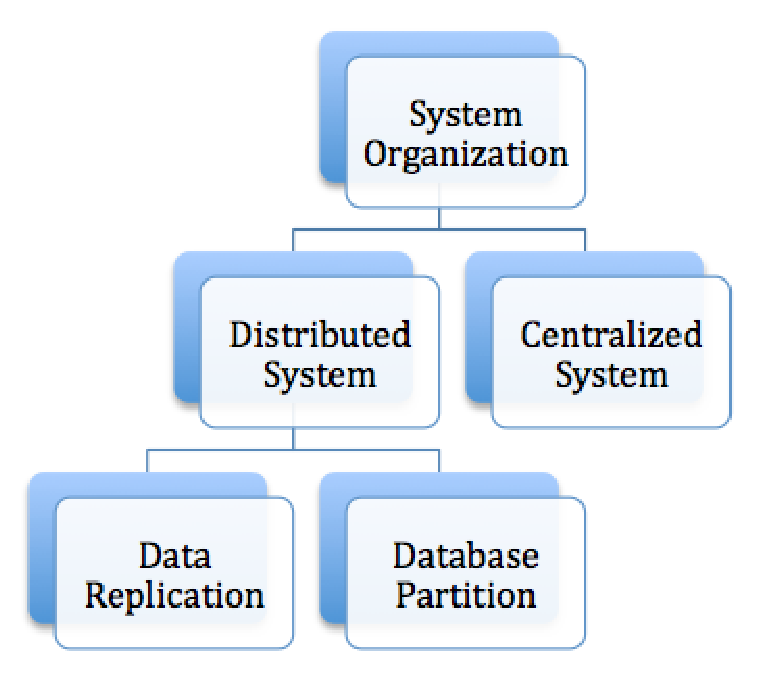
\includegraphics{../diagrams/taxonomy-database-architecture}
  \caption{Database Architecture Taxonomy}
  \label{fig:taxonomy-database-architecture}
\end{figure}

\begin{itemize}
  \item \textbf{Centralized System}: a database system that runs in one single
  centralized host, being the focal purpose of data traffic as read and writes 
  \cite{sn-intro01};
  \item \textbf{Distributed System}: a database system that can be composed by
  more than one node. Usually, the use of the pattern of Master-Slave
  mechanism or data ``Replication" is used. Another mechanism is the use of
  database paritioning, if the technology supports it.
\end{itemize}

\section{Relationships among the Taxonomies}

The different taxonomies defined in the previous sections of this chapter are
important to the understanding of a data persistence layer for sensor
networks. As they are closely related to each other, it is important to
briefly highlight these relationships in order to better analyze a problem
related to data persistence. 

The taxonomy related to the purpose of the sensor data can be directly related
to the taxonomy of the location of the sensor data. While the taxon of the 
real-time data stream relates to the local data storage, the taxon related to
data archival correlates the storage of the collected data into an external
storage. In addition to that, the converse is also true.

The taxonomy related to the data model can be related to any taxon from the
taxonomy of the location of the sensor data, as well as the taxons related to
Data Provenance. In the former, the data of a relational model is stored using
SQL messages.

In the light of these taxonomies, the classification of the data persistence
properties of a sensor networks can be studied and reviewed. As described in
the introduction of this dissertation, one the main motivations for this work
was to provide means of data persistence of NetBEAMS, a case study which does
not contain a data layer. Therefore, the following chapter seeks to describe
that case study in order to make a section of a given technology for evaluation.
